\section{Movimiento Rectilíneo Uniformemente Variado:}
 
En este movimiento al contrario que el MRU la velocidad con la que se mueve el móvil ya no es constante en el tiempo, y existe 
una nueva cantidad cinemática que da de cuenta de este cambio llamada \textit{aceleración}. 

\subsection{La aceleración:}

La aceleración $a$ es una cantidad vectorial que mide el ritmo de cambio de la velocidad con respecto al tiempo. Es decir, esta 
cantidad es una medida de como cambia la velocidad del móvil. Y esta cantidad se calcula así:

\begin{equation}
 \vec{a}=\frac{\Delta \vec{v}}{\Delta t}\quad [m/s^2] 
 \end{equation}
 
siendo $\Delta \vec{v}=\vec{v_f}-\vec{v_0}$ la diferencia entre velocidades (desde una velocidad inicial $\vec{v_0}$ hasta una 
velocidad final $\vec{v_f}$) realizado por el cuerpo en el intervalo de tiempo $\Delta t$.\\

La principal característica del MRUV es que posee una aceleración que es constante en el tiempo, es decir, la aceleración del 
cuerpo con MRUV siempre tendrá el mismo valor para cualquier instante de tiempo. Por ejemplo la caída libre de un cuerpo, con 
aceleración de la gravedad constante.\\

El movimiento rectilíneo uniformemente variado puede ser acelerado o desacelerado (retardado):\\

\textbf{Acelerado:} El movimiento es acelerado cuando la aceleración que experimenta el cuerpo en movimiento es de signo positivo 
($a > 0$), y esto quiere decir que con el paso del tiempo el cuerpo se ``acelera'': su velocidad va aumentando en el tiempo.\\

\textbf{Retardado:} Es cuando la aceleración que experimenta el cuerpo en movimiento es de signo negativo ($a < 0$), y esto 
quiere decir que con el paso del tiempo el cuerpo se ``desacelera'' o se ?frena?: su velocidad va disminuyendo en el tiempo.\\

\begin{figure}[ht]
 \centering
 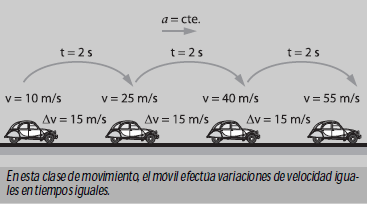
\includegraphics[scale=0.7]{images/mruv.png}
 % cinematica.png: 0x0 px, 300dpi, 0.00x0.00 cm, bb=
 \caption{Ilustración de una automóvil con MRUV.}\label{mruv}
\end{figure} 

En la figura \ref{mruv} se observa como un automóvil con MRUV cada 2 segundos incrementa su velocidad en $\Delta v = 15 m/s$, y 
así por tanto su aceleración es $a = \frac{\Delta v}{\Delta t} = \frac{15 m/s}{2s} = 7.5 m/s^2$, y como en este caso como $a>0$ 
se trata de un movimiento acelerado.\\

Este movimiento esta regido por cuatro ecuaciones de movimiento siguientes:

\begin{equation}
 v_f = v_o + at
\end{equation}

\begin{equation}
 v_f^2 = v_0^2 + 2ad
\end{equation}

\begin{equation}
 d = (\frac{v_f+v_0}{2})t
\end{equation}

\begin{equation}
 d = v_0t+ \frac{1}{2}at^2
\end{equation}

Dónde: $v_f$ : es la velocidad final del cuerpo en movimiento (se mide en $[m/s]$), $v_0$ : es la velocidad inicial del cuerpo en 
movimiento (se mide en $[m/s]$), $a$ : es la aceleración del cuerpo en movimiento (se mide en $[m/s 2]$), $t$: es el tiempo que 
emplea el cuerpo durante el movimiento (se mide en $[s]$), d: es la distancia recorrida por el cuerpo (se mide en $[m]$). Estas 
ecuaciones están planteadas de forma escalar, es decir, relacionan los módulos de las magnitudes vectoriales del cuerpo en 
movimiento, pero es importante notar que estas ecuaciones también se pueden plantear de forma vectorial de la siguiente manera: 

\begin{equation}
\vec{v_f} = \vec{v_0} + \vec{a}t 
\end{equation}

\begin{equation}
 v_f^2 = v_0^2+2a\Delta r
\end{equation}

\begin{equation}
 \Delta \vec{r} = (\frac{\vec{v_f}+\vec{v_0}}{2})t
\end{equation}

\begin{equation}
 \Delta \vec{r} = \vec{v_0}t + \frac{1}{2}\vec{a}t^2
\end{equation}
 
Observando detenidamente estas ecuaciones se infiere que cada ecuación tiene cuatro diferentes magnitudes relacionadas 
a través de ella, y por tanto conocer cualquiera de ella está en función de las otras tres, es decir, es suficiente con 
este tipo de ecuaciones encontrar una magnitud conociendo otras tres distintas (este es un dato importante en el momento de 
resolver problemas relacionados con el MRUV).

\subsection{Problemas de mruv}

\begin{enumerate}
 \item Un ciclista que está en reposo comienza a pedalear hasta alcanzar los 6 m/s en 6 minutos. Calcular la distancia total que 
recorre si continúa acelerando durante 5 minutos más.

\item  Un cuerpo se mueve con una velocidad de $3 \vec{i} – 4\vec{j}$ [m/s] y
 se le aplica una aceleración de $0.3 m/s^2$

 en la misma dirección de la velocidad. Determine la
 distancia recorrida al cabo de un minuto de recorrido.

 
\item Dos vehículos separados por 20 km parten al encuentro
 en el instante t=0. El primero lo hace con una velocidad inicial 
constante de 20 km/h. El
 segundo parte desde el reposo y con una aceleración de $0,5 m/s^2$. ¿A qué distancia de la
 salida del 
primer vehııculo se encuentran? 

\item Un móvil viaja a 60 km/h y comienza a reducir su velocidad a partir del instante t=0. Al
 cabo de 8 segundos se detiene 
completamente. ¿Cuál fue aceleración durante el período en el que redujo su
 velocidad?

\item Un tren viaja a 80 km/h. Inmediatamente después de pasar una señal en rojo comienza a
 detenerse. Se detiene completamente 
a los 150 metros. Determinar su aceleración.

\item Un automóvil corre a una velocidad 
 de 20 m/s, en ese instante pisa el acelerador produciendo una aceleración constante 
que aumenta 
su velocidad a 30 m/s en 5s. ¿Cuál será su velocidad al cabo de 10s?

\item Un móvil se desplaza con velocidad inicial desconocida. A partir de t=0 comienza a acelerar
 a $1,7 m/s^2$
. Luego de 12 
segundos se desplaza a 110 km/h. Determinar la velocidad inicial.

\item Un tren viaja a una velocidad constante de 90 km/h y pasa una señal en rojo. A 80 metros
 de pasar la señal comienza a 
reducir su velocidad a razón de $3m/s^2$
. ¿A qué distancia de la señal se detiene
 por completo?¿Cuánto tarda en hacerlo a 
partir del momento en el que pasa la señal?

\item Dos vehículos separados por 20 km parten al encuentro en el instante t=0. El primero lo
 hace con una velocidad inicial 
constante de 20 km/h. El segundo parte desde el reposo y con una aceleración
 de $0,5 m/s^2$
 . ¿A qué distancia de la salida 
del primer vehículo se encuentran?

\item Dos vehículos A y B se mueven con aceleración
 constante, el vehículo B tiene una velocidad inicial $\vec{v_0B} = (50 
\vec{i} – 4 \vec{j}) km/h$, y después de 2
 horas alcanza una velocidad final $\vec{v_fB}=(54 \vec{i} + 16\vec{j}) km/h$. Si se 
conoce que la aceleración
 del vehículo A es el doble que la del vehículo B, determine la aceleración del vehículo A.



\end{enumerate}
